\subsection{Polarized Target}
\label{POLTARGSEC}
This experiment will use the
JLab/UVa dynamically polarized solid {\TARGET}target operated in longitudinal mode.  
%Transverse polarization requires  operation of an upstream chicane to ensure proper transport through the target magnetic field.  
The target is typically operated with a specialized slow raster, and beamline instrumentation capable of characterizing the low current 50-100 nA beam.
All of these requirements have been met previously in Hall C.
%, and will be soon implemented also in Hall A for the E08-027/E08-007 run in 2011. 
%
The polarized target (see Fig.~\ref{fig:target}), 
has been successfully used in experiments E143, E155, and E155x at SLAC, and E93-026, E01-006 and E07-003, E08-027 and E08-007 at JLab.
A similar target was used in Hall B for the EG1,EG4 and DVCS experiments. 
%although Hall B does
%not at present have the facilities necessary to operate a transversely polarized target with an electron beam.

The JLAb/UVa target underwent significant renovation and improvement~\cite{CKEITH} during the recent g2p run. The magnet was replaced early in the run, and the target then performed consistently at or above historical levels.   A new 1 K refrigerator and target insert were designed and constructed by the JLab target group.  The cryogenic pumping system has been overhauled.  In particular, the older Alcatel 2060H rotary vane pumps have been replaced with new Pfeiffer DU065 magnetically coupled rotary vane pumps, and the pump controls are being refurbished. The target motion system has been rebuilt from scratch. %And now, the magnet and vacuum jacket rotate independently of the refrigerator and target insert, which simplifies rotation from parallel to perpendicular magnetic field orientations.

%
\begin{figure}
\centering
%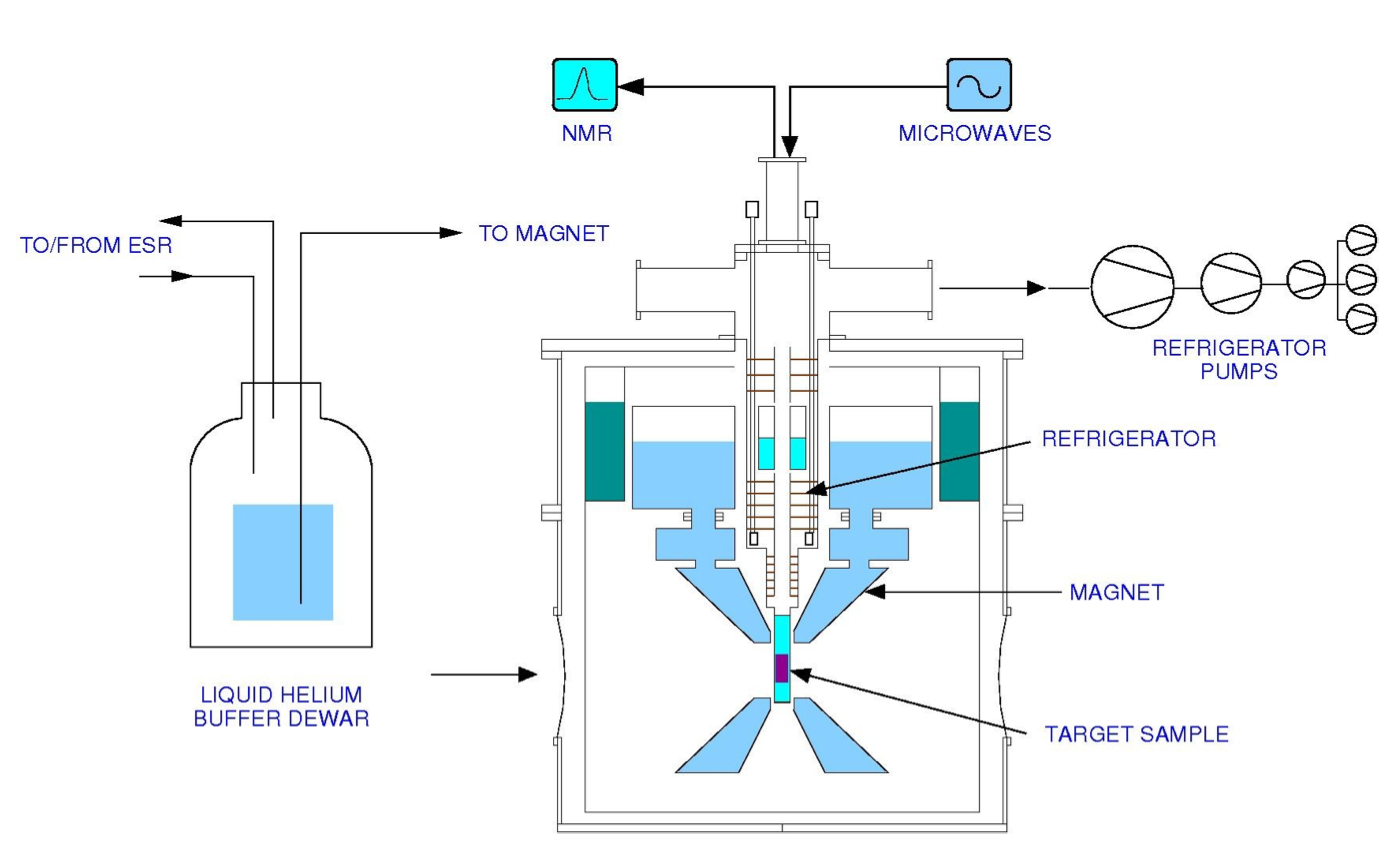
\includegraphics[width=5.0in,clip]{figs/targnew.eps} %target_gimp.eps}
\caption{Cross section view of the JLab/UVa polarized target. Figure courtesy of C. Keith.  \label{fig:target}}
\end{figure}


%\begin{figure}
%\centering
%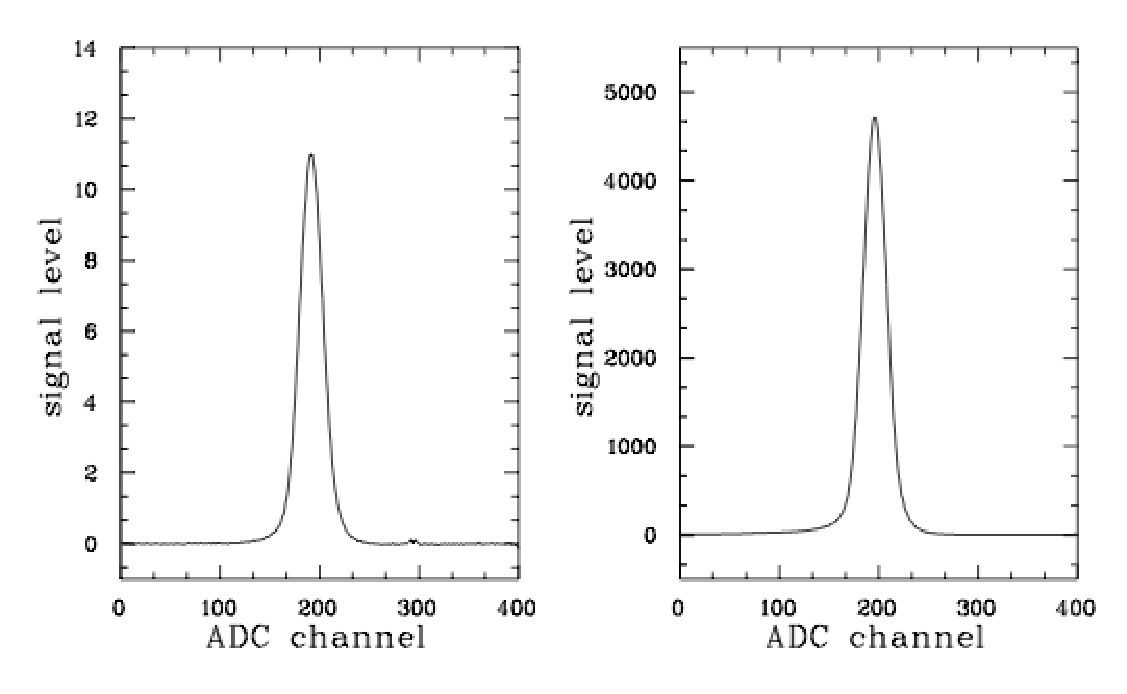
\includegraphics[width=4.5in,clip]{figs/liD.eps}
%\caption{\label{fig:LID} Typical Deuteron thermal equilibrium (TE) and enhanced signals in $^6$LiD.  The left plot shows a typical deuteron TE and the right shows an enhanced deuteron NMR signal.  Note its clean undistorted shape unlike for $^{15}ND_3$.  Also, note the scale difference between the TE and enhanced signals.
%{\it Reproduced from Ref.~\cite{ALTOBIAS}}.}
%\end{figure}

\begin{figure}
\centering
%\includegraphics[width=0.5\textwidth]{figs/tensor_pol3.eps}
\caption{{\bf Top}: NMR signal for ND$_3$ with a vector polarization of approximately 50\% from the GEN experiment.  %The average polarization in beam for that experiment was 35\%. 
{\bf Bottom}: Relationship between vector and tensor polarization in equilibrium, and 
neglecting the small quadrupole interaction.  \label{fig:tensorpol}}
\end{figure}

\begin{figure}
\centering
%\includegraphics[width=3.0in,clip]{figs/gen.eps} %target_gimp.eps}
\caption{Performance of the ND$_3$ target during the GEN experiment.  \label{fig:gen}}
\end{figure}


The target operates on the principle of Dynamic Nuclear Polarization, to
enhance the low temperature (1 K), high magnetic field (5 T) polarization of solid
materials  by microwave pumping.
The polarized target assembly contains several target cells of 3.0 cm length
that can be  selected individually by remote control to be located in the uniform field
region of a superconducting Helmholtz pair. The permeable target cells are
immersed in a  vessel filled with liquid Helium and maintained at 1 K by use of a
high power evaporation refrigerator.
The coils have a 50$^\circ$ conical shaped aperture along the beam axis
which allow for unobstructed forward scattering.
%34$^\circ$ wedge shaped aperture along the vertically oriented midplane.

The target material is exposed to microwaves
to drive the hyperfine transition which  aligns the nucleon spins. 
 The heating of the target by the beam causes a drop of a few percent in
the polarization, and the polarization slowly decreases with time due to radiation
damage. Most of the radiation damage can be repaired by periodically annealing the target,
until the accumulated dose reached is greater than about 
%$ 17\times 10^{15}$ e$^-$/cm$^2$, 
 $0.5\times 10^{17}$ e$^-$/cm$^2$,
at
which time the target material needs to be replaced. 
%The luminosity of the polarized 
%material in the uniform field region is approximately $85\times 10^{33}$ cm$^{-2}$ Hz.

\subsubsection{Polarization Analysis} 
%Eq.~\ref{TENSORVECTOR} allows calculation of a target's tensor polarization once the vector polarization has been determined.  
The three Zeeman sublevels of the deuteron system ($m=-1,0,1$) are
shifted unevenly due to the quadrupole interaction~\cite{Meyer:1985dta}. This shift
depends on the angle between the magnetic field and the electrical field gradient, and gives rise to two separate transition
energies. Hence, the unique double peaked response displayed in Fig.~\ref{fig:tensorpol}.
When the system is at thermal equilibrium with the solid lattice, the deuteron polarization is known from:
\begin{eqnarray}
\label{VECT}
P_z = \frac{4+\tanh\frac{\mu B}{2 k T}} {3+\tanh^2\frac{\mu B}{2 k T}    }
\end{eqnarray}
where $\mu$ is the magnetic moment, and $k$ is Boltzmann's constant.  The vector polarization can be determined by comparing
the enhanced signal with that of the TE signal (which has known polarization).  This polarimetry method is typically reliable to about 5\% relative.

Similarly, the tensor polarization is given by: 
\begin{eqnarray}
\label{TENS}
P_{zz} = \frac{4+\tanh^2\frac{\mu B}{2 k T}} {3+\tanh^2\frac{\mu B}{2 k T}    }
\end{eqnarray}

From Eqs.~\ref{VECT} and~\ref{TENS}, we find:
\begin{eqnarray*}
\label{PZZEQN}
P_{zz}= 2 - \sqrt{4-3 P_z^2}
\end{eqnarray*}


In addition to the TE method, polarizations can be determined by analyzing NMR lineshapes as described in~\cite{Dulya:1997qc} with a typical  7\% relative uncertainty.  At high polarizations, the
intensities of the two transitions differ, and the NMR signal shows an asymmetry R in the
value of the two peaks, as shown in Fig.~\ref{fig:tensorpol}.  The vector polarization is then given by:
\begin{eqnarray}
\label{RVECT}
P_{z} = \frac{R^2-1}{R^2+R+1}
\end{eqnarray}
and the tensor polarization is given by:
\begin{eqnarray}
\label{TVECT}P_{zz} = \frac{R^2-2 R +1}{R^2+R+1}
\end{eqnarray}


%or by comparison of the NMR response to the known thermal equilibrium (TE) polarization with typical 5\% uncertainty.

The DNP technique produces  deuteron vector polarizations of up to 60\%  in ND$_3$ 
and 64\% in LiD~\cite{Bueltmann:1998wq}, which corresponds to tensor polarizations of approximately 30\%.
%Tensor polarizations of 22\% have been achieved in previous experiments~\cite{Meyer:1985dta}
%using standard solid polarized ammonia targets.
The target polarization decays while in beam, so that the average vector polarization 
was about 35\% in the GEN experiment, as seen if Fig.~\ref{fig:gen}.

%While it is not necessary for this experiment, it may be possible to directly determine the tensor polarization directly from the analyzing power T$_{20}$


An average tensor polarization of \PZZ\% enables a significant measurement of $b_1(x)$, as shown in 
Fig.~\ref{PROJ}.  Any improvement to the expected polarization, although not strictly necessary, 
would allow the addition of kinematic points, and/or improved statistical accuracy.
With this in mind, we are pursuing techniques to enhance the tensor polarization by directly stimulating 
transitions to/from the $M_s=0$ state, as discussed in Ref.~\cite{Meyer:1985dta}.  D. Crabb from the UVa group  
had some success in obtaining enhanced tensor polarizations via RF saturation of one of the Zeeman transitions, otherwise known as ``hole-burning''.  The method was not pursued due to the
lack of need for tensor polarized targets at the time of the study.  Another method to enhance tensor polarization entails simultaneously pumping the sample with two independent microwave frequencies, 
which requires careful isolation of the respective cavities. 
%We reiterate that the rates in this proposal assume only polarizations that have been demonstrated previously during typical operation at JLab.


\subsubsection{Depolarizing the Target}
%The NMR will be used on both to probe polarization.  
To move from polarized to unpolarized measurements, the target
polarization will be annihilated using destructive NMR loop field changes and destructive DNP microwave pumping.
It is also possible to remove LHe in the nose of the target to remove the polarization by heating.
During unpolarized data taking the incident electron beam heating is enough to remove the thermal equilibrium polarization.

The NMR measurement will ensure zero polarization.  The target material will be
kept at $\sim$1 K for polarized and unpolarized data collection, and the target field
will be held constant for both states as well.  These
consistencies are used to minimize the systematic differences in the
polarized and unpolarized data collection.  To minimize systematic effects over
time, the polarization condition will be switched twice in a 24 hour period. 
This is expected to account for drift in integrated charge accumulation.

%(I think we should move this discussion to another section dealing with target
%physics and the overhead time accounting. Also,  I would favor dumping the LHe, and refilling the
%nose.)}


\subsubsection{Rendering Dilution Factor}
\label{dil}
To derive the dilution factor, we first start with the ratio of 
polarized to unpolarized counts.
%equation used to obtain the observable in terms of each measured cross section.
%\begin{equation}
%\frac{A_{zz}P_{zz}}{2}=\left(\frac{\sigma^1-\sigma}{\sigma}\right).
%\end{equation}
In each case, the number of counts that are actually measured,  neglecting 
the small contributions of the thin aluminium cup window materials, NMR coils, etc.,
are
\begin{equation}
N_1=Q_1\varepsilon_1 {\cal A}_1 l_1[(\sigma_N+3\sigma_1)p_f+\sigma_{He}(1-p_f)],
\end{equation}
and
\begin{equation}
N=Q\varepsilon {\cal A}l[(\sigma_N+3\sigma)p_f+\sigma_{He}(1-p_f)].
\end{equation}
where $Q$ represents accumulated charge, $\varepsilon$ is the dectector 
efficiency, ${\cal A}$ the cup acceptance, and $l$ the cup length.  

For
this calculation we assume similar charge accumulation such that $Q\simeq Q_1$, 
and that the efficiencies stay constant, in which case all factors drop out of 
the ratio leading to
\begin{eqnarray}
\nonumber \frac{N_1}{N}& = &\frac{{(\sigma_N+3\sigma_1)p_f+\sigma_{He}(1-p_f)}
}{(\sigma_N+3\sigma)p_f+\sigma_{He}(1-p_f)}\\
\nonumber & = & \frac{{(\sigma_N+3\sigma(1+A_{zz}P_{zz}/2))p_f+\sigma_{He}(1-p_
f)}}{(\sigma_N+3\sigma)p_f+\sigma_{He}(1-p_f)}\\
\nonumber & = & \frac{{[(\sigma_N+3\sigma)p_f+\sigma_{He}(1-p_
f)]+3\sigma A_{zz}P_{zz}/2}}{(\sigma_N+3\sigma)p_f+\sigma_{He}(1-p_f)}\\
\nonumber & = & 1 + \frac{3\sigma 
A_{zz}P_{zz}/2}{(\sigma_N+3\sigma)p_f+\sigma_{He}(1-p_f)}\\
& = & 1 + \frac{1}{2} f A_{zz}P_{zz}, 
\end{eqnarray}
where $\sigma_1 = \sigma(1+A_{zz}P_{zz}/2)$ has ben substituted, per 
Eq.~\ref{eq:one}, with $P_B =0$. It can be seen that the above result 
corresponds to Eq.~\ref{3}.

